\documentclass[aspectratio=169]{beamer}
\usetheme{metropolis} 
% \usetheme[progressbar=frametitle]{metropolis}
\usepackage{appendixnumberbeamer}
 
\usepackage{booktabs}
\usepackage[scale=2]{ccicons}

\usepackage{xspace}
\newcommand{\themename}{\textbf{\textsc{metropolis}}\xspace}

\usepackage[backend=biber,doi=true, natbib=true,style=ieee ]{biblatex}
\addbibresource{main.bib}

\title{Earth at night}
\subtitle{The visualisation of average radiance in 3 areas}
\date{\today}
% \date{}
\author{Zhen Chen (John)}
\institute{A2 Inc}
\titlegraphic{\hfill
\includegraphics[height=1.5cm]{images/logo.png}}

\begin{document}

\maketitle

\begin{frame}{}
  \setbeamertemplate{section in toc}[sections numbered]
  \tableofcontents[hideallsubsections]
\end{frame}

\section{Introduction of the background}

\begin{frame}[fragile]{Background: World Bank Nightime Light Data}

  \begin{columns}
    \column{0.5\textwidth}
    World Bank Nightime Light Data consists of a lot of satellite imagery 
    stored in Amazon Web Services (AWS) (Fig.~\ref{wbs3}). 
    
    Latest files from 2012 to 2020 are generated by the sensor 
    named Visible Infrared Imaging Radiometer Suite Day-Night Band (VIIRS DNB) \citep{WorldBan13:online}.
    
    \column{0.5\textwidth}
      \begin{figure}[htbp]
        \centerline{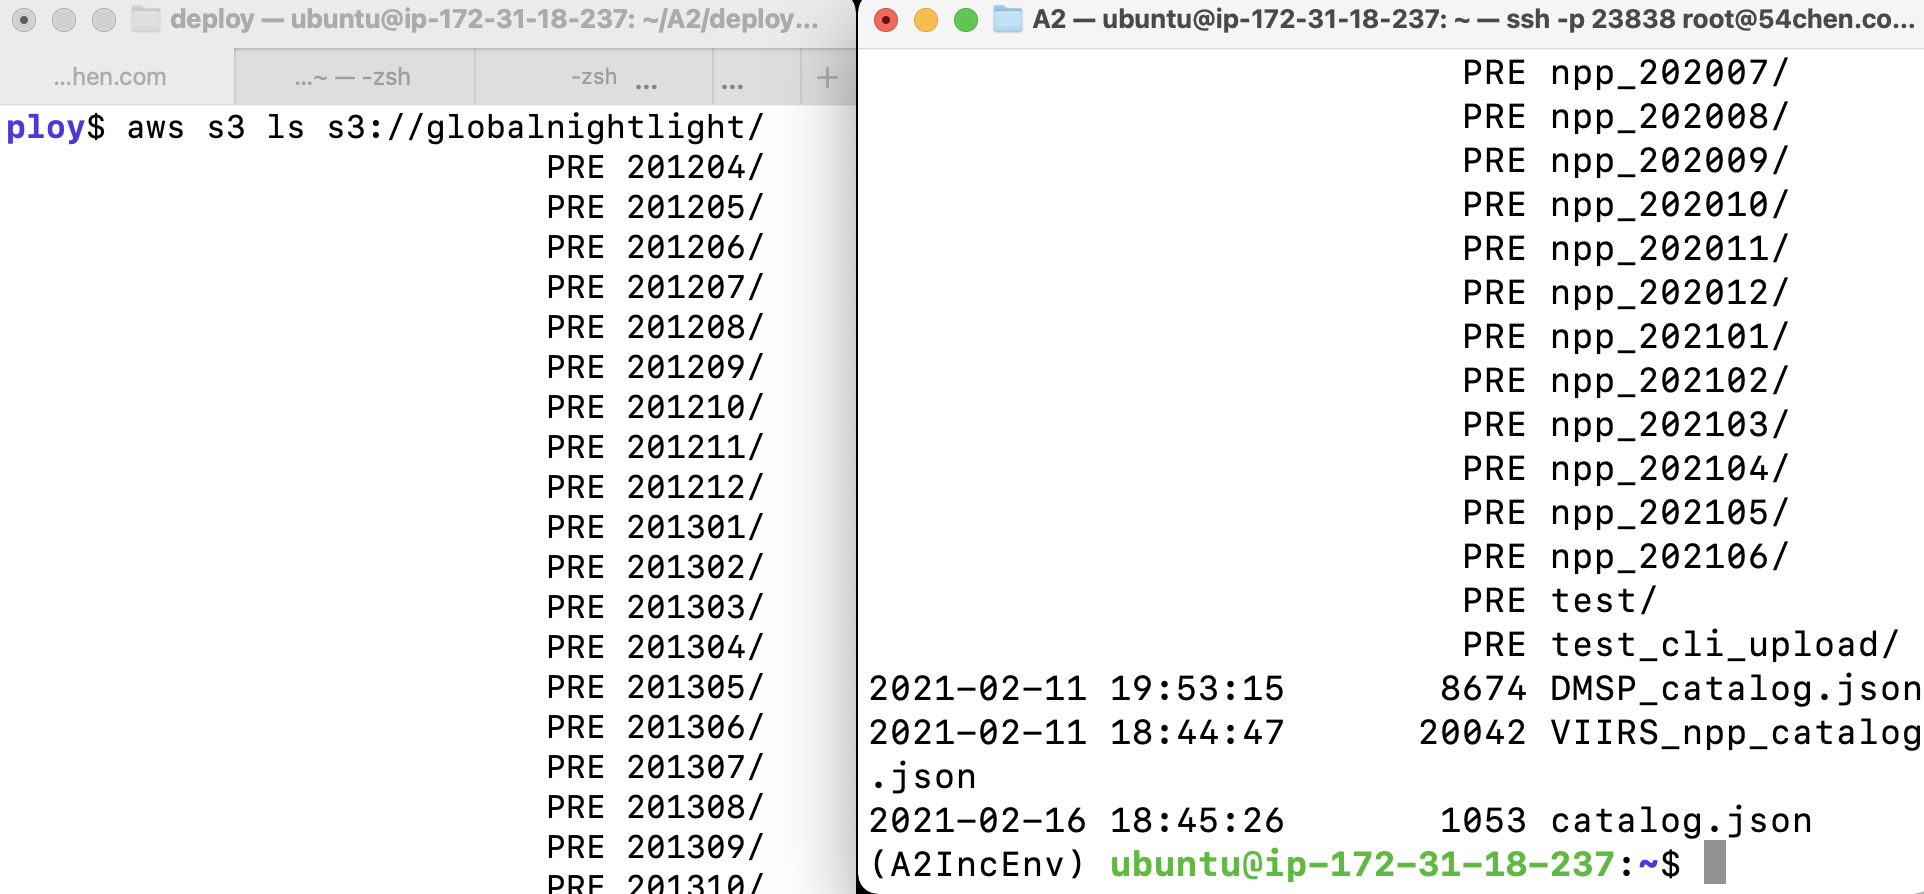
\includegraphics[width=200pt]{images/3.1.png}}
        \caption{World Bank Nighttime Light Data}
        \label{wbs3}
      \end{figure}
    \end{columns}
  \end{frame}
  
\begin{frame}[fragile]{Background: COG}

  \begin{columns}
    \column{0.5\textwidth}
    
    \begin{figure}[htbp]
      \centerline{
\includegraphics[width=200pt]{images/youtube.png}}
      \caption{COG}
      \label{youtube}
    \end{figure}

    \column{0.5\textwidth}
    All imagery is stored in S3 by Cloud Optimized GeoTIFF (COG) \citep{CloudOpt5:online}.
  \end{columns}
\end{frame}

\begin{frame}[fragile]{Background: STAC}

  \begin{columns}
    \column{0.5\textwidth}
    
    \begin{figure}[htbp]
      \centerline{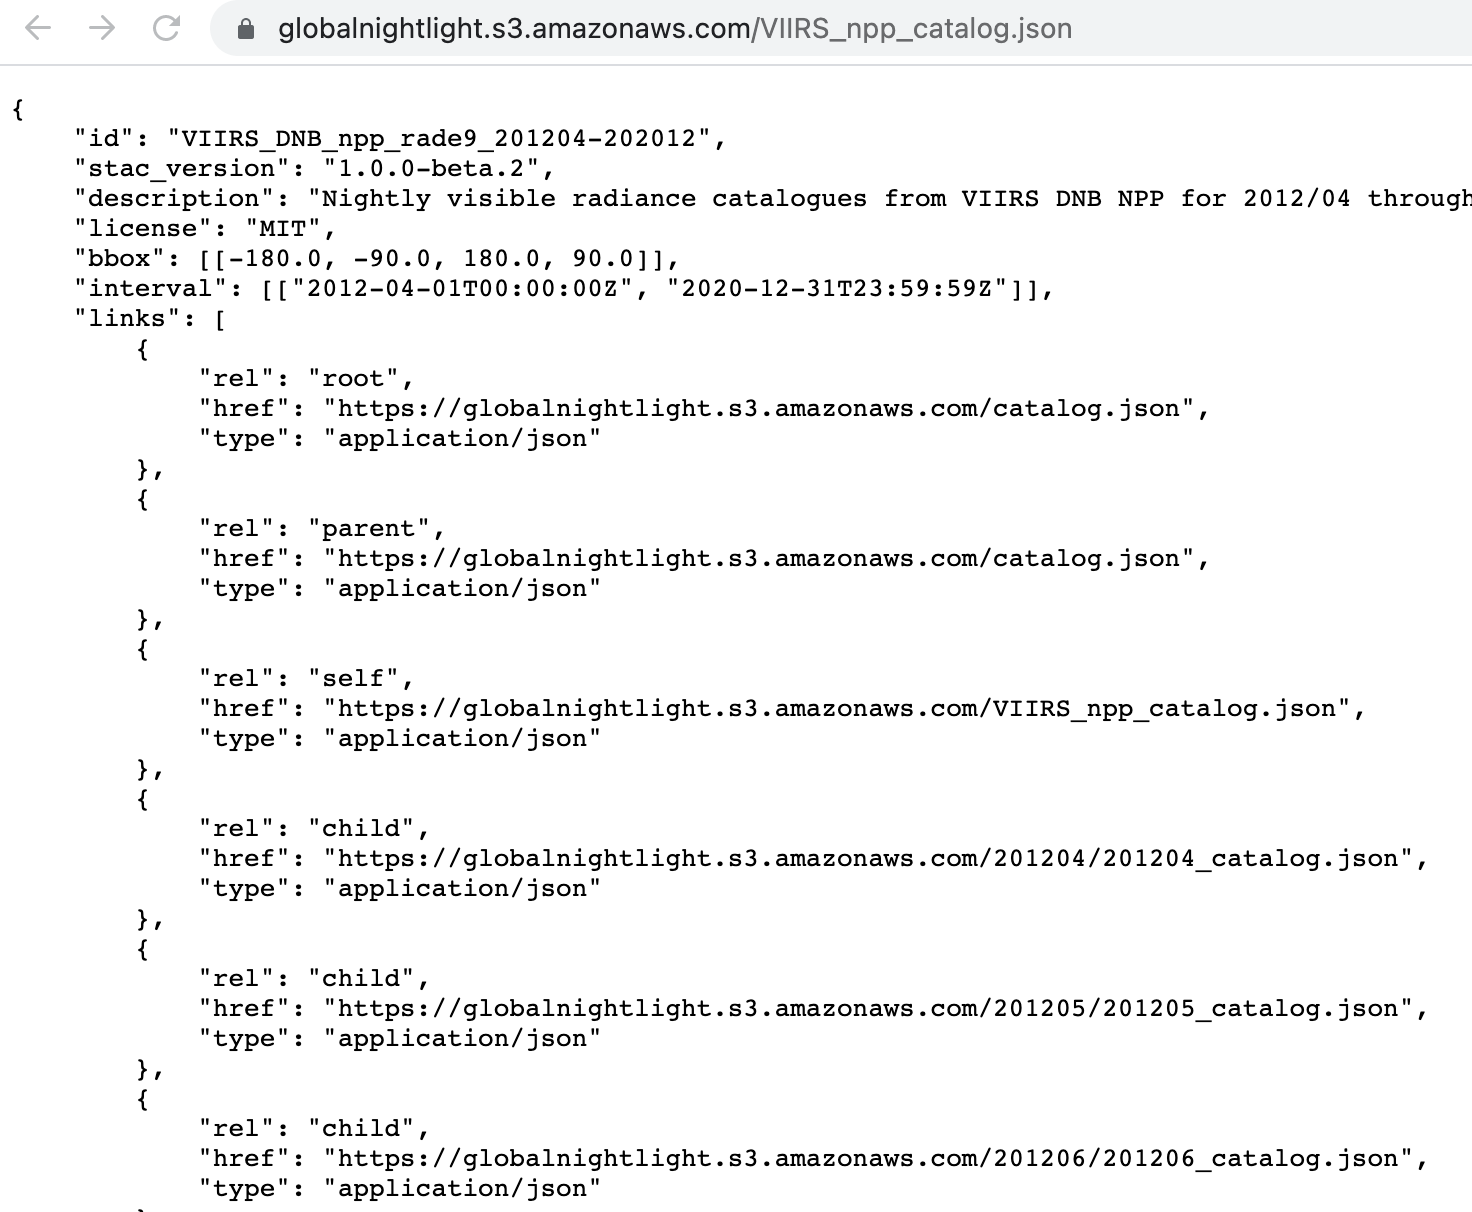
\includegraphics[width=170pt]{images/STAC.png}}
      \caption{STAC of Global ngiht lights}
      \label{STAC}
    \end{figure}

    \column{0.5\textwidth}
    All of the imagery and metadata is organized by Spatial Temporal Asset Catalog (STAC) \citep{SpatioTe90:online}. 
  \end{columns}
\end{frame}

\begin{frame}[fragile]{Background: Objective}

  \begin{columns}
    \column{0.5\textwidth}
    Our objective is to build a demo to show the ngihttime lights status in 3 specific areas.
    \column{0.5\textwidth}
      \begin{figure}[htbp]
        \centerline{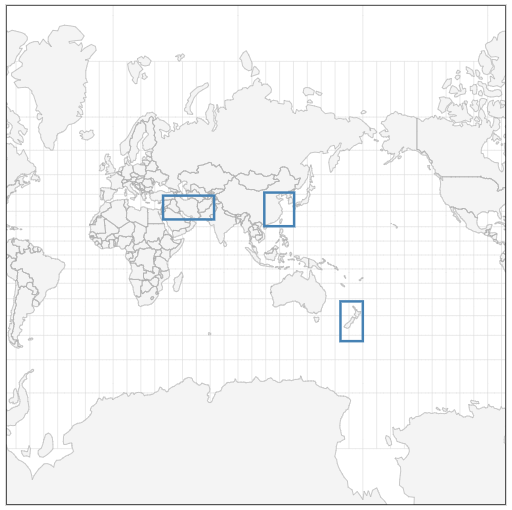
\includegraphics[width=140pt]{images/Worldmap.png}}
        \caption{3 areas we researched}
        \label{areas}
      \end{figure}
  \end{columns}
\end{frame}

\section{Architecture}

\begin{frame}[fragile]{AWS}

  
  \begin{figure}[htbp]
    \centerline{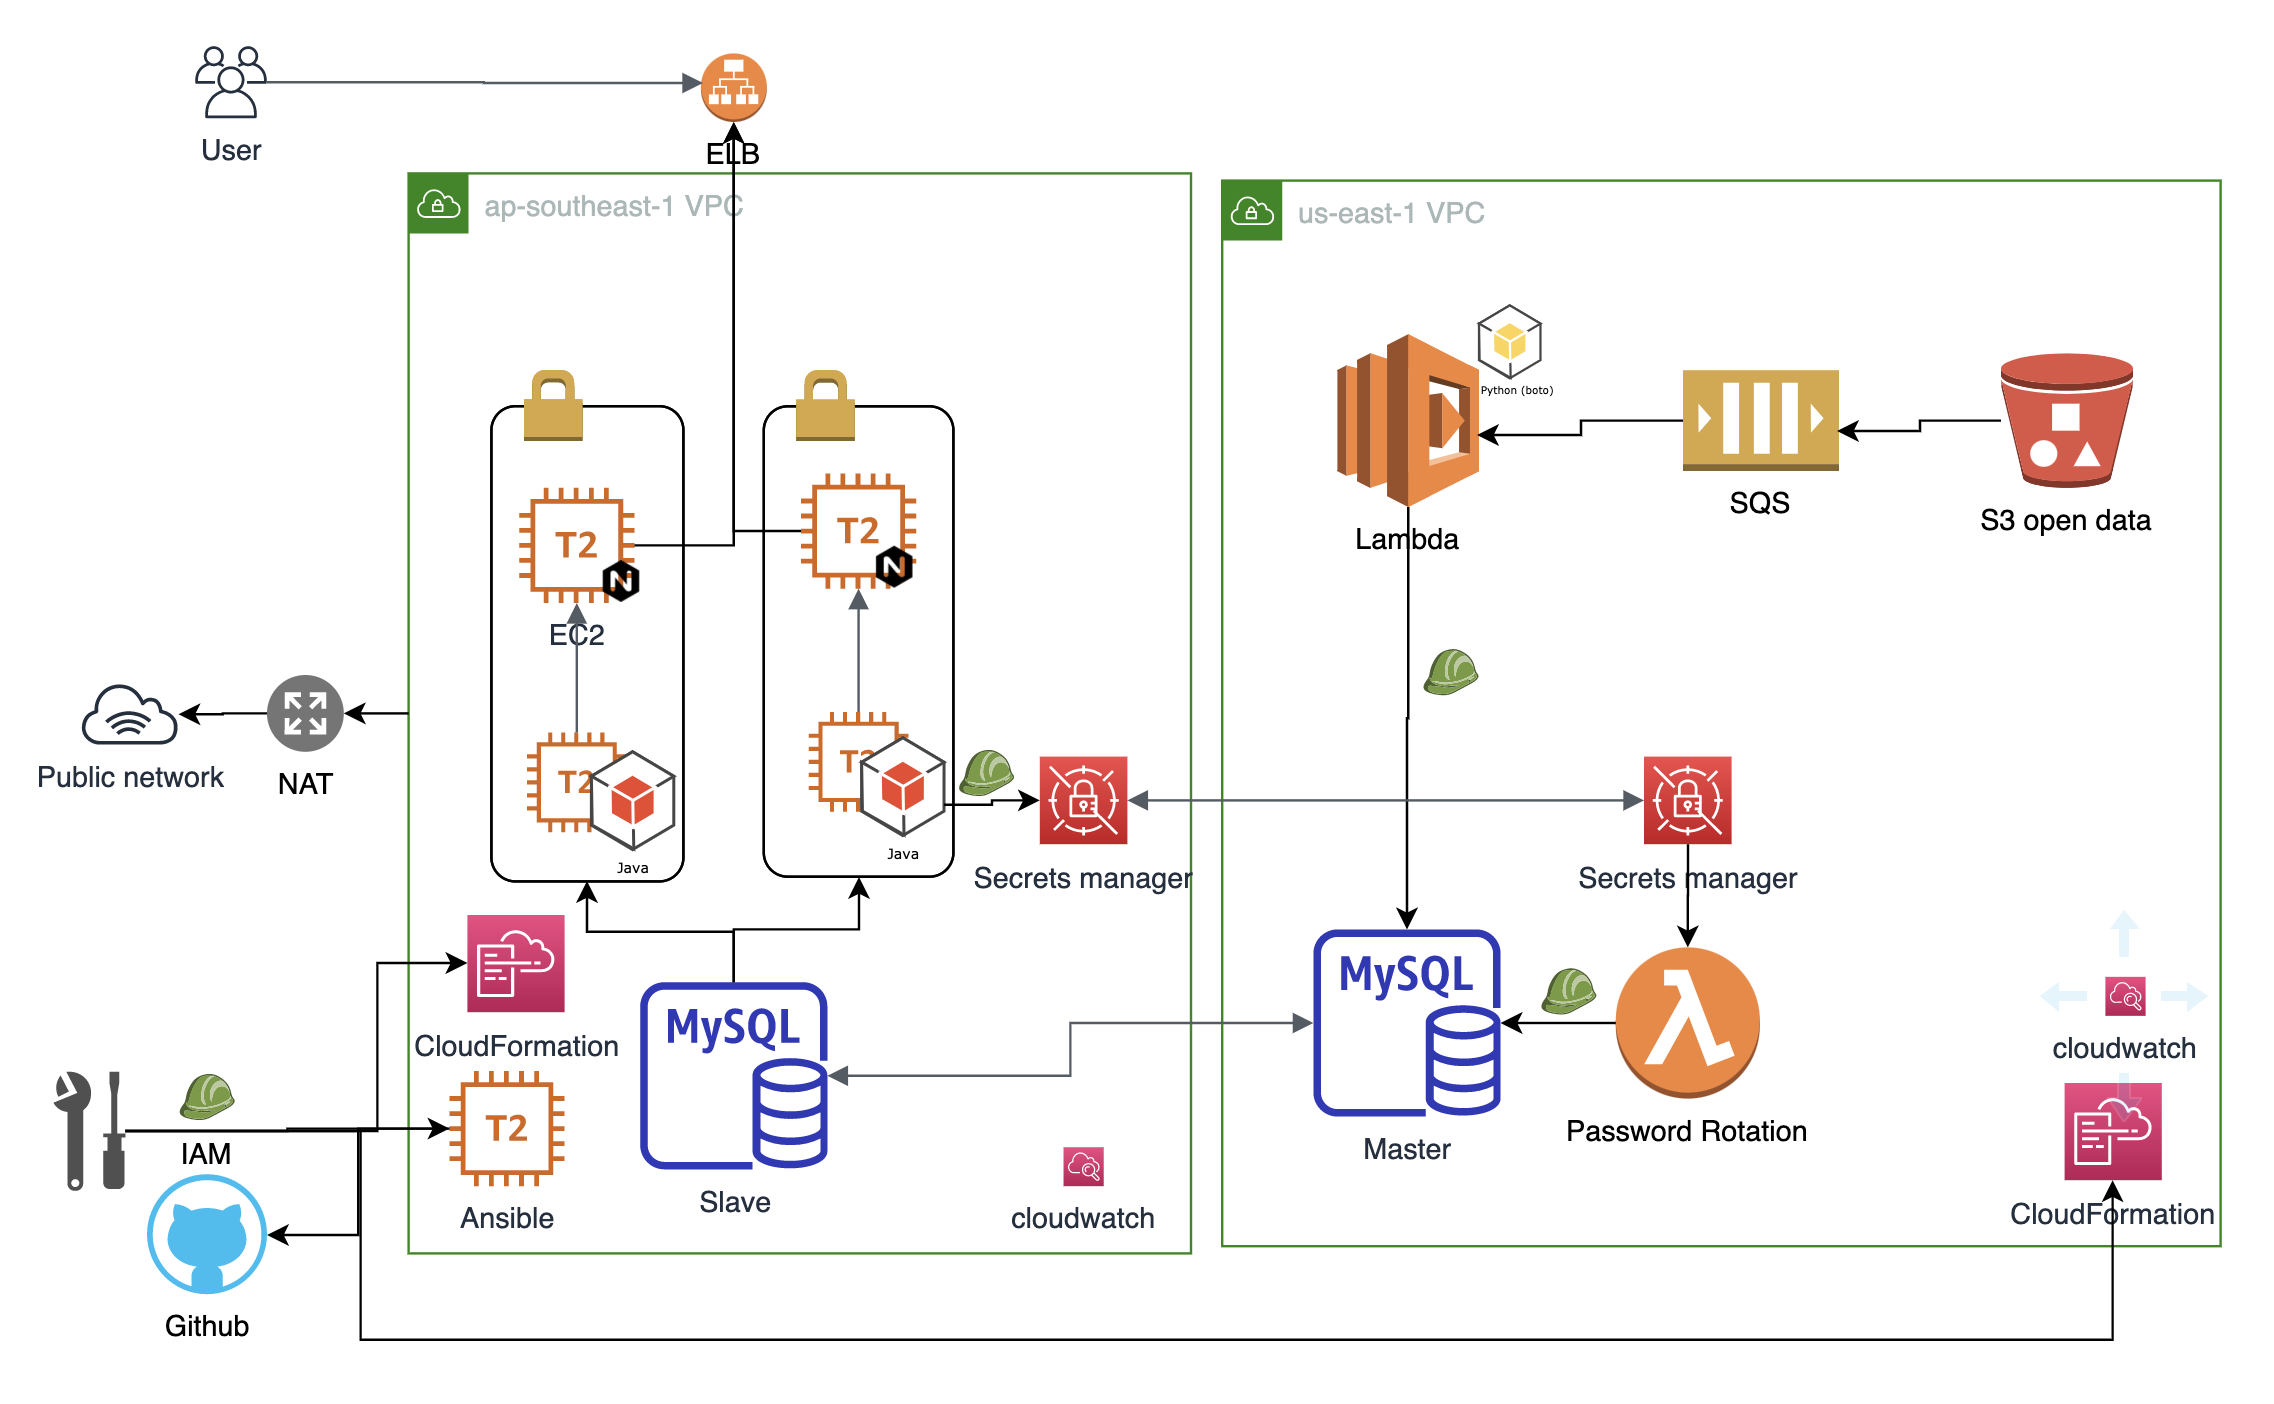
\includegraphics[width=260pt]{images/arch.png}}
    \caption{Architecture}
    \label{fig2}
  \end{figure}

\end{frame}

\begin{frame}[fragile]{Services}

  \begin{itemize}
    \item EC2
    \item RDS
    \item Lambda
  \end{itemize}

\end{frame}

\begin{frame}[fragile]{security implementation}

  \begin{itemize}
    \item IAM
    \item network
    \item data security
  \end{itemize}

\end{frame}

\section{Security}

\begin{frame}[fragile]{security implementation}

  \begin{itemize}
    \item IAM
    \item network
    \item data security
  \end{itemize}

\end{frame}

\section{Reference}

\begin{frame}[allowframebreaks]{Reference}

   \printbibliography[heading=none]
 
\end{frame}

\end{document}